\documentclass[modern]{aastex62}

% lsstdoc documentation: https://lsst-texmf.lsst.io/lsstdoc.html
\input{meta}

% Package imports go here.

% Local commands go here.



\newcommand{\docRef}{PSTN-052}
\newcommand{\docUpstreamLocation}{\url{https://github.com/lsst-pst/pstn-052}}


\begin{document}
\input{authors}
\date{\today}
\title{Survey Strategy: Rolling Cadence}
\hypersetup{pdftitle={\@title}, pdfauthor={\@author}, pdfkeywords={\@keywords}}

\begin{abstract}
here's an abstract
\end{abstract}

\section{Introduction}

Motivation for rolling cadence:  The SRD says the WFD region should have 825 visits (spread over the ugrizy filters) after 10 years. This works out to one observation every 4.4 days (or one observation every 3.3 days if we have a 9-month observing season). For many transient phenomenon, including SNe Ia, this cadence is not ideal and something slightly higher (e.g., one observation every 2 days) would be preferred.

There is no free lunch. Going to higher cadence at one time demands that there be a corresponding time of lower cadence. In Figure~\ref{fig:ideal_foot} we show the ideal cumulative number of observations for different observing strategies. The cadence one can request is highly constrained. For one, we desire the final survey to be uniform, so all the strategies need to end at the same level. If one wants to include an increased cadence, that necessarily means that point in the sky will also need to have a corresponding period of lower cadence. Similarly, if a point has a higher cadence, another point at similar RA must also have a lower cadence (we cannot increase the observing cadence simultaneously everywhere).



\begin{figure}
\plotone{plots/footprint_ideal.pdf}
\caption{A comparison of how the cumulative number of observations varies at 4 points in the sky and for non-rolling and rolling cadences. \label{fig:ideal_foot}}
\end{figure}

\begin{figure}
\plotone{plots/actual_footprint.pdf}
\caption{\label{fig:actual_foot}}
\end{figure}

Some limitations we have on rolling cadence:

The Science Requirements Document (SRD) places tight constraints on how well Rubin must be able to measure the proper motion on stars. The uncertainty on proper motion is dominated by the baseline of the observations--namely, it is optimal to have observations spaced as far apart as possible. This means we need to maximize the number of observations taken in the first and last observing seasons for every point in the sky. Since the SRD requirement applies to the entire WFD region, this essentially means we need to have even sky coverage (no rolling) at the start and end of the survey. 

When the survey begins, there will be a region of sky already partially though it's observing season. Thus, we need to observe with a uniform cadence for 1.5 years at the start and end of the survey. If we observe for 1.5 years uniform at the start, we must also observe for 1.5 years at the end. That leaves 7 potential years for rolling. 


Another limitation is ensuring we have adequate images to construct image difference templates. 

Yet another potential limitation is the nature of the Rubin alert stream. If we construct the rolling cadence such that we concentrate observations on the southern sky for a year, that will mean the alert stream will be concentrated in the southern sky, and a large fraction of potential follow-up facilities (those in Hawaii and the American SW) will be unable to participate in transient follow-up for an entire year. Having multiple declination bands for rolling also helps the scheduler work around lunar avoidance.



Rolling introduces a number of free parameters
\begin{itemize}
    \item{How strong should the rolling be?}
    \item{Do we want to have repeat visits (beyond a pair) in a night?}
    \item{Do we want to encourage/discourage nightly cadence?}
    \item{What should the footprint be?}
    \item{How many rolling bands should there be?}
\end{itemize}
The dimensionality of the problem is clearly an issue.


For the scheduler, we define a footprint object that computes desired fraction of observations that a point on the sky should receive as function of time. Each filter has it's own footprint object. In Figure XXX, we plot the results of this footprint object for a single point on the sky.




\section{Lots of plots}

\begin{figure}
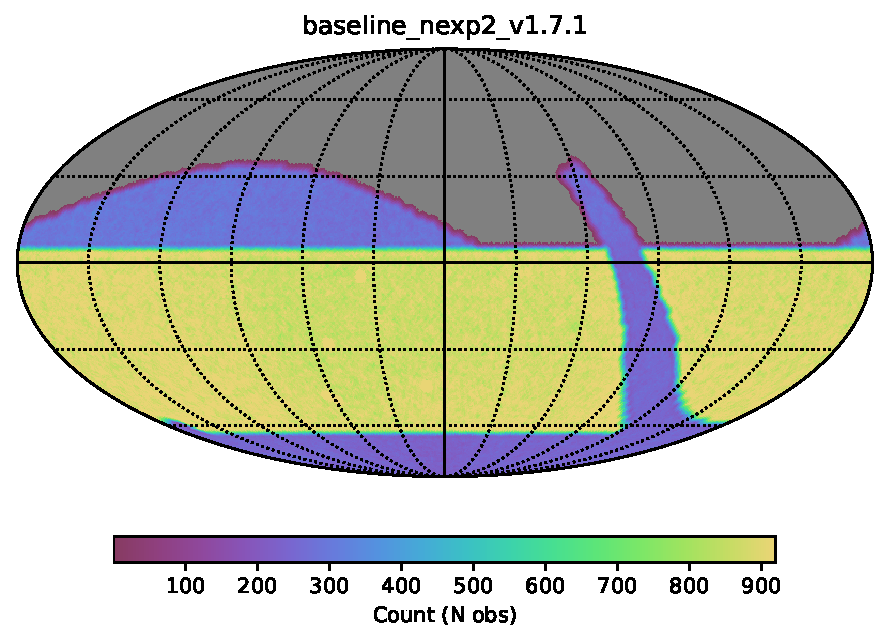
\includegraphics[height=1.25in, width=1.75in]{plots/baseline_nexp2_v1.7.1/baseline_nexp2_v1_7_1_Count_HEAL_SkyMap.pdf}
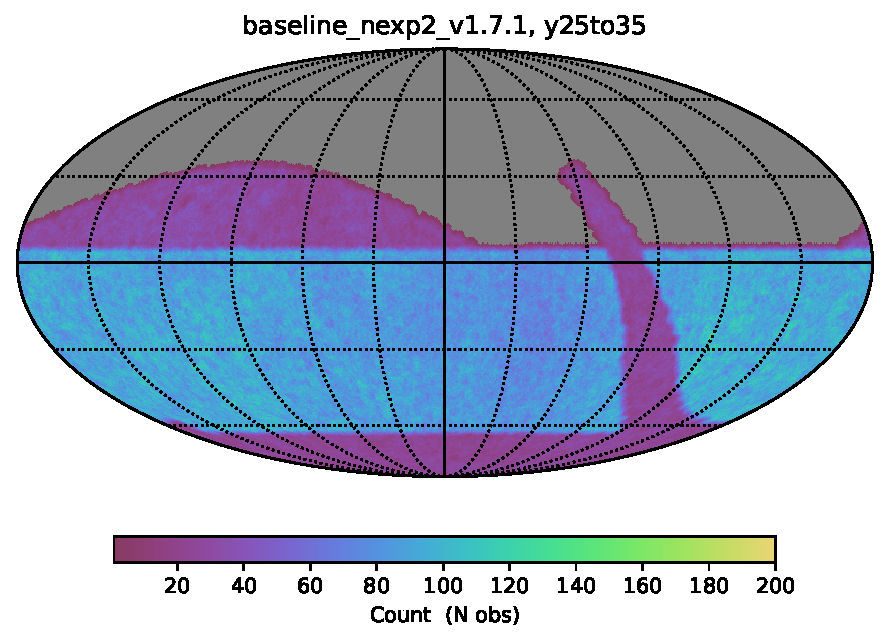
\includegraphics[height=1.25in, width=1.75in]{plots/baseline_nexp2_v1.7.1/baseline_nexp2_v1_7_1_Count_night_gt_913_125000_and_night_lt_1278_375000_and_note_not_like_DD_HEAL_SkyMap.pdf}
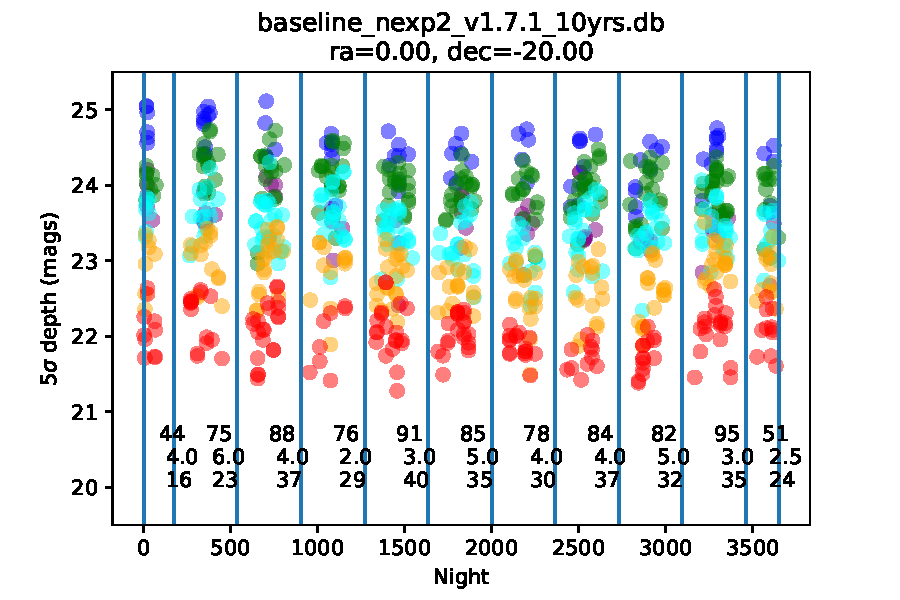
\includegraphics[height=1.25in, width=1.75in]{plots/baseline_nexp2_v171_spotc.pdf}\\
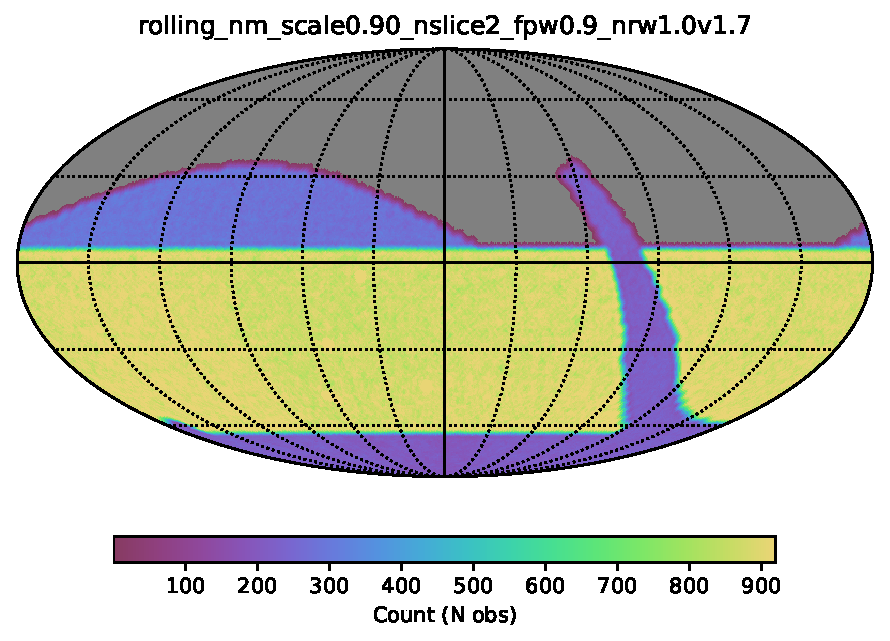
\includegraphics[height=1.25in, width=1.75in]{plots/rolling_nm_scale0.90_nslice2_fpw0.9_nrw1.0v1.7/rolling_nm_scale0_90_nslice2_fpw0_9_nrw1_0v1_7_Count_HEAL_SkyMap.pdf}
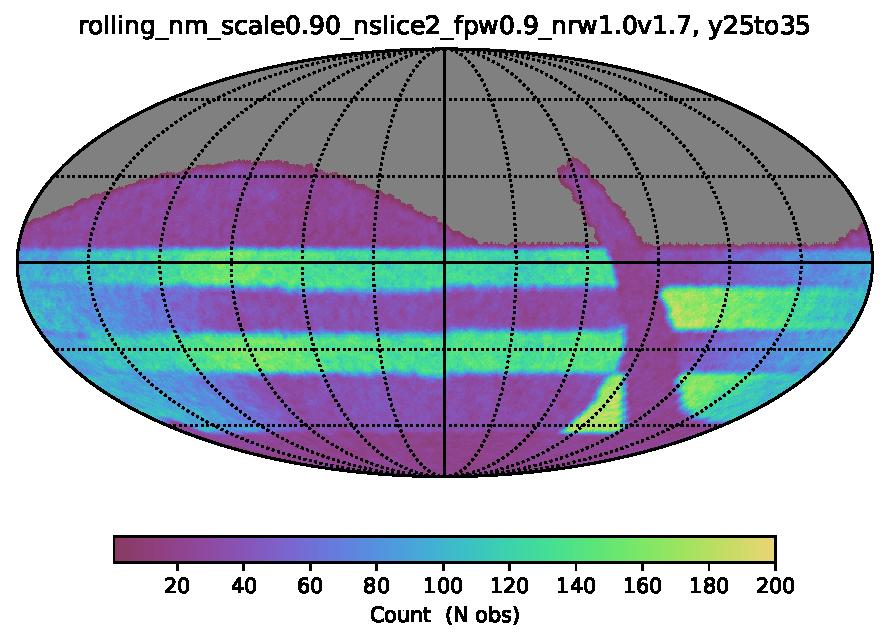
\includegraphics[height=1.25in, width=1.75in]{plots/rolling_nm_scale0.90_nslice2_fpw0.9_nrw1.0v1.7/rolling_nm_scale0_90_nslice2_fpw0_9_nrw1_0v1_7_Count_night_gt_913_125000_and_night_lt_1278_375000_and_note_not_like_DD_HEAL_SkyMap.pdf}
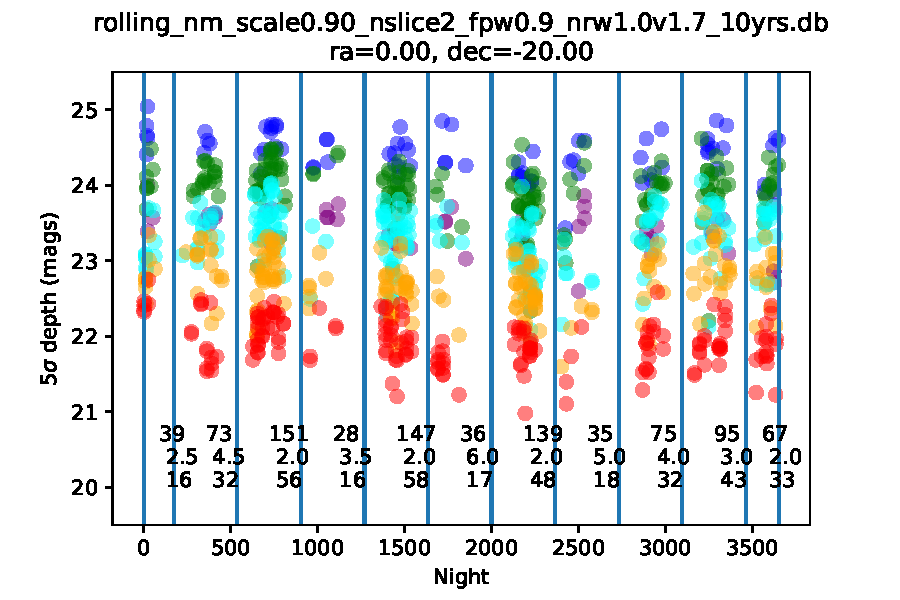
\includegraphics[height=1.25in, width=1.75in]{plots/rolling_nm_scale090_nslice2_fpw09_nrw10v17_spotc.pdf}\\
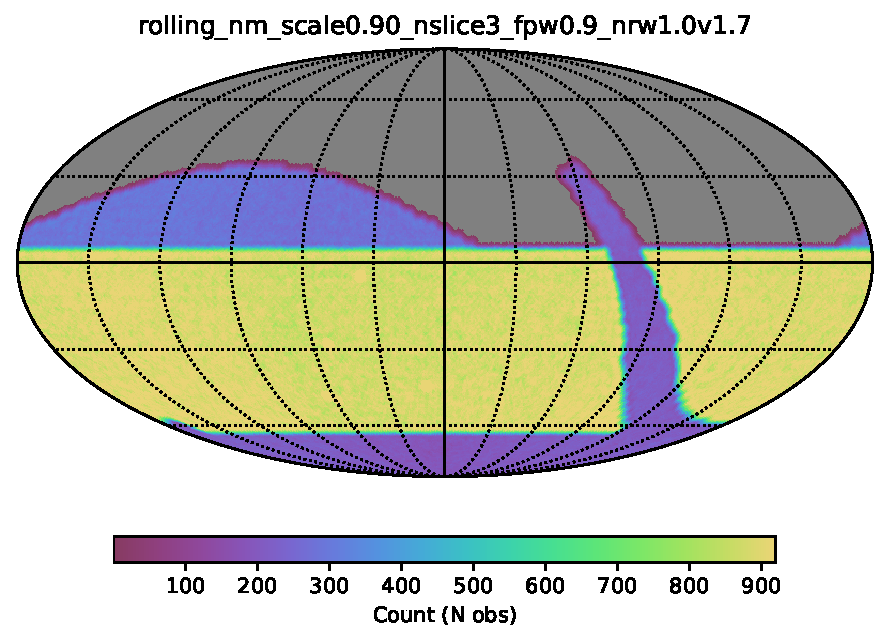
\includegraphics[height=1.25in, width=1.75in]{plots/rolling_nm_scale0.90_nslice3_fpw0.9_nrw1.0v1.7/rolling_nm_scale0_90_nslice3_fpw0_9_nrw1_0v1_7_Count_HEAL_SkyMap.pdf}
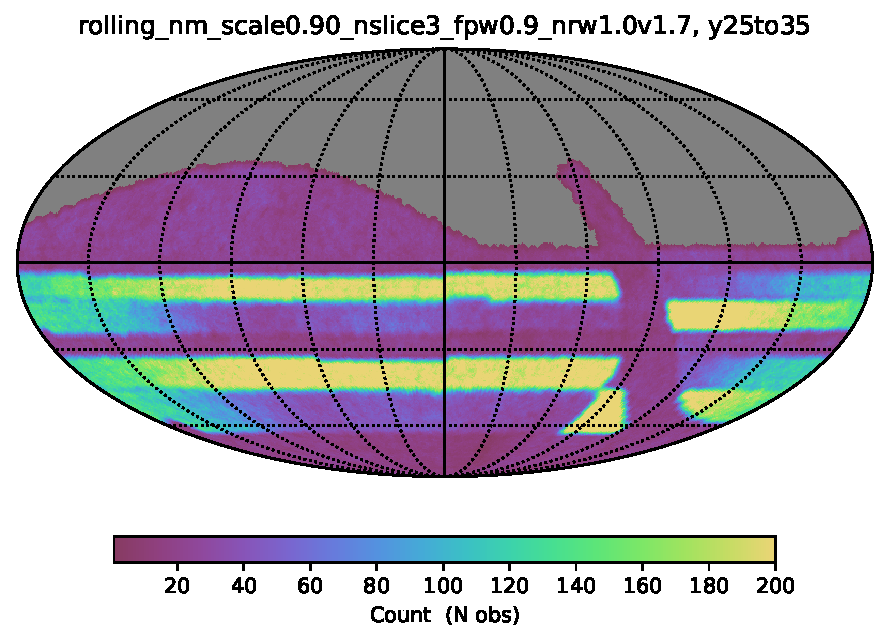
\includegraphics[height=1.25in, width=1.75in]{plots/rolling_nm_scale0.90_nslice3_fpw0.9_nrw1.0v1.7/rolling_nm_scale0_90_nslice3_fpw0_9_nrw1_0v1_7_Count_night_gt_913_125000_and_night_lt_1278_375000_and_note_not_like_DD_HEAL_SkyMap.pdf}
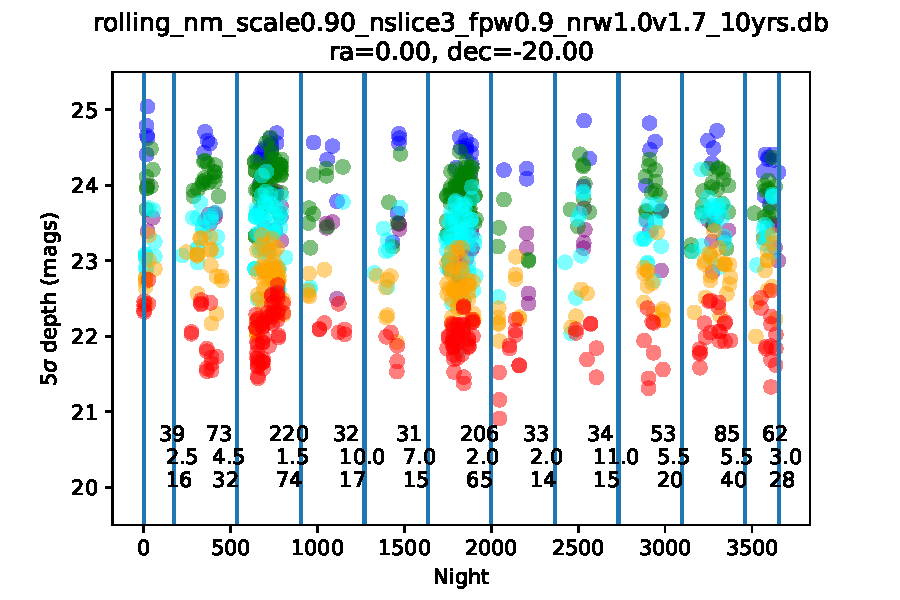
\includegraphics[height=1.25in, width=1.75in]{plots/rolling_nm_scale090_nslice3_fpw09_nrw10v17_spotc.pdf}
\caption{Plots showing the results for various simulations with the classic survey footprint. On the left, we plot the total number of observations (all filters) after 10 years. Middle panels show non-deep drilling observations taken between years 2.5 and 3.5. Right panels show observations that overlap a sample point at RA=0, dec=-20. Horizontal lines denote different observing seasons, with annotations for the total number of observations in a season, median gap between days that have an observation, and the total number of days in the season with an observation. The top shows the baseline strategy, middle a rolling cadence where half the sky is rolling for three on and three off seasons, bottom shows a rolling cadence where one third of the sky is on for two seasons and off for four seasons. \label{fig:classics}}
\end{figure}



\begin{figure}
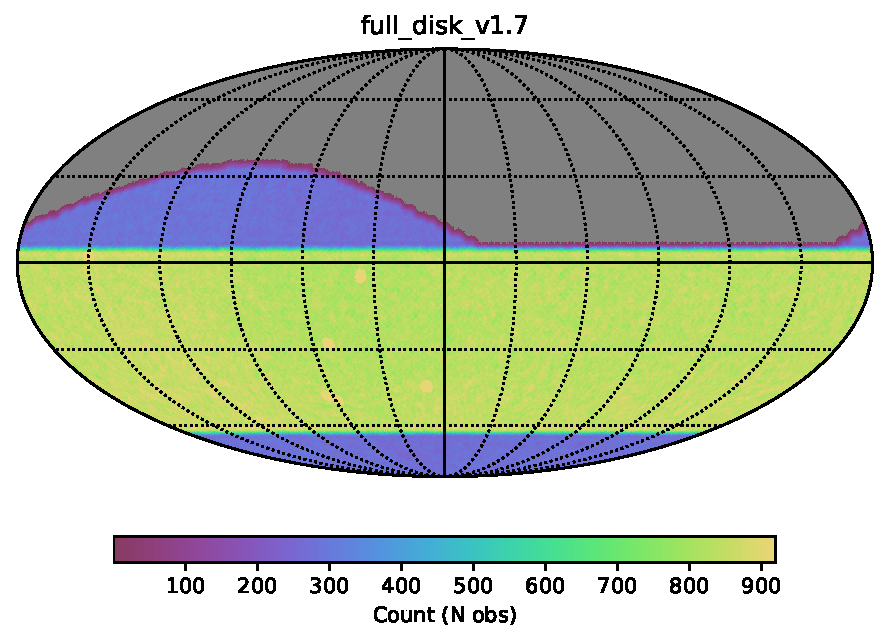
\includegraphics[height=1.25in, width=1.75in]{plots/full_disk_v1.7/full_disk_v1_7_Count_HEAL_SkyMap.pdf}
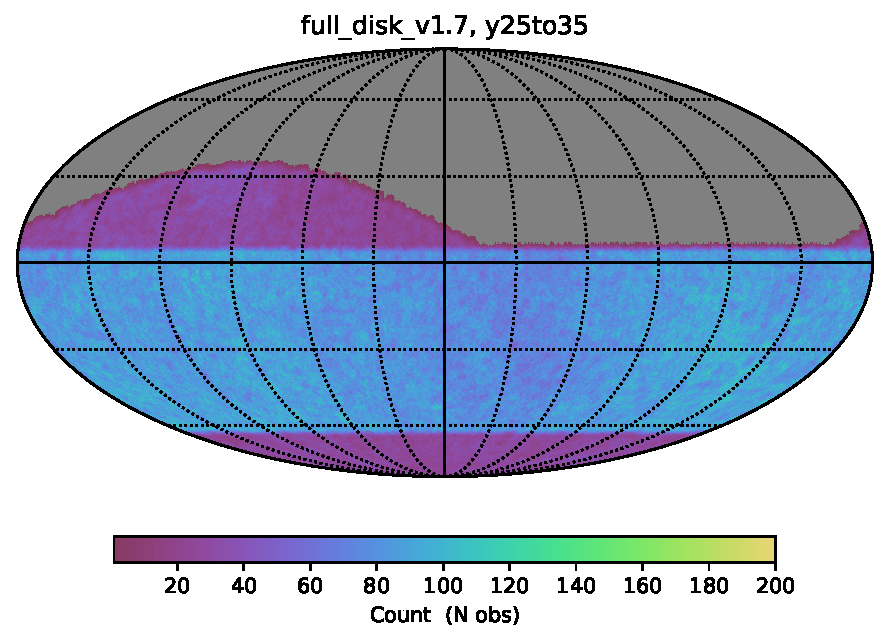
\includegraphics[height=1.25in, width=1.75in]{plots/full_disk_v1.7/full_disk_v1_7_Count_night_gt_913_125000_and_night_lt_1278_375000_and_note_not_like_DD_HEAL_SkyMap.pdf}
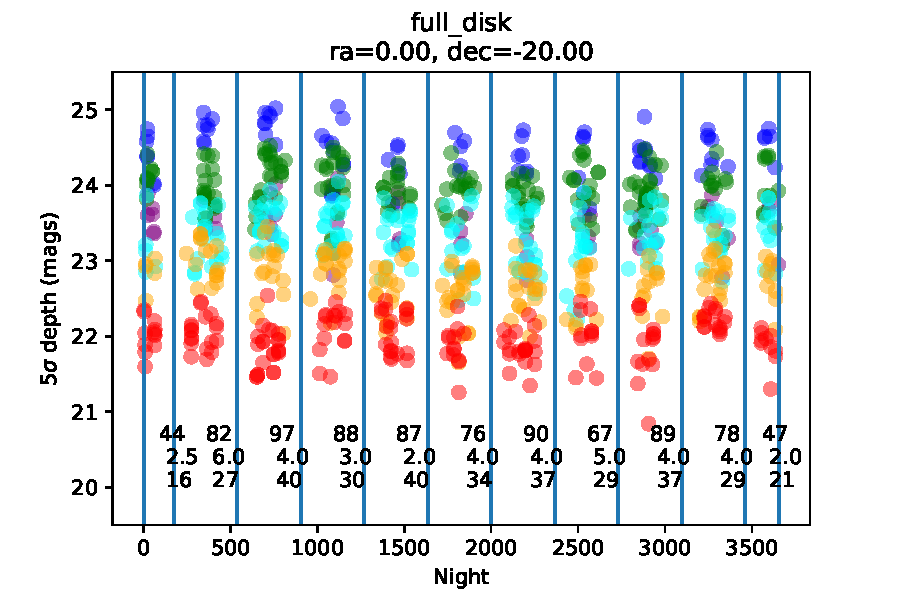
\includegraphics[height=1.25in, width=1.75in]{plots/full_disk_v17_spotc.pdf} \\
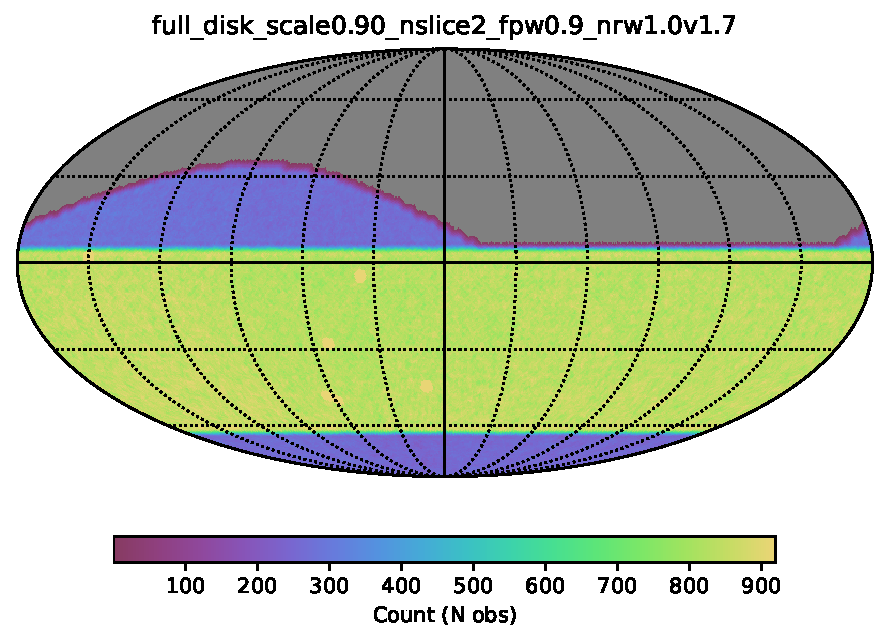
\includegraphics[height=1.25in, width=1.75in]{plots/full_disk_scale0.90_nslice2_fpw0.9_nrw1.0v1.7/full_disk_scale0_90_nslice2_fpw0_9_nrw1_0v1_7_Count_HEAL_SkyMap.pdf}
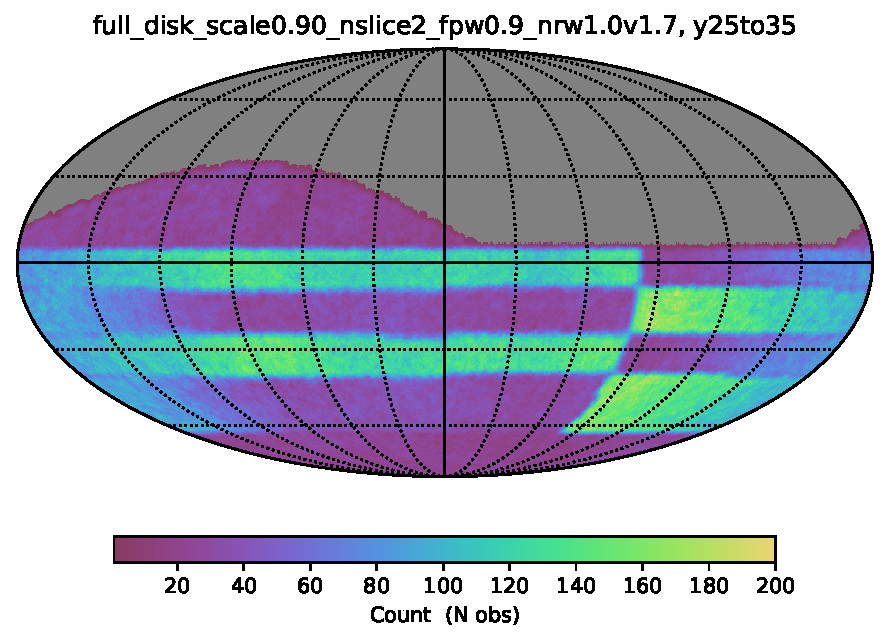
\includegraphics[height=1.25in, width=1.75in]{plots/full_disk_scale0.90_nslice2_fpw0.9_nrw1.0v1.7/full_disk_scale0_90_nslice2_fpw0_9_nrw1_0v1_7_Count_night_gt_913_125000_and_night_lt_1278_375000_and_note_not_like_DD_HEAL_SkyMap.pdf}
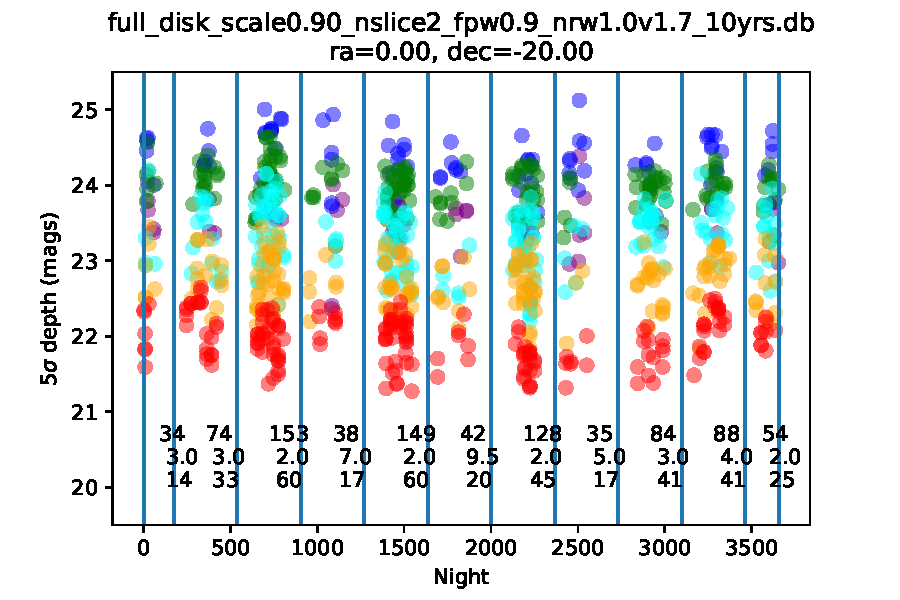
\includegraphics[height=1.25in, width=1.75in]{plots/full_disk_scale090_nslice2_fpw09_nrw10v17_spotc.pdf} \\
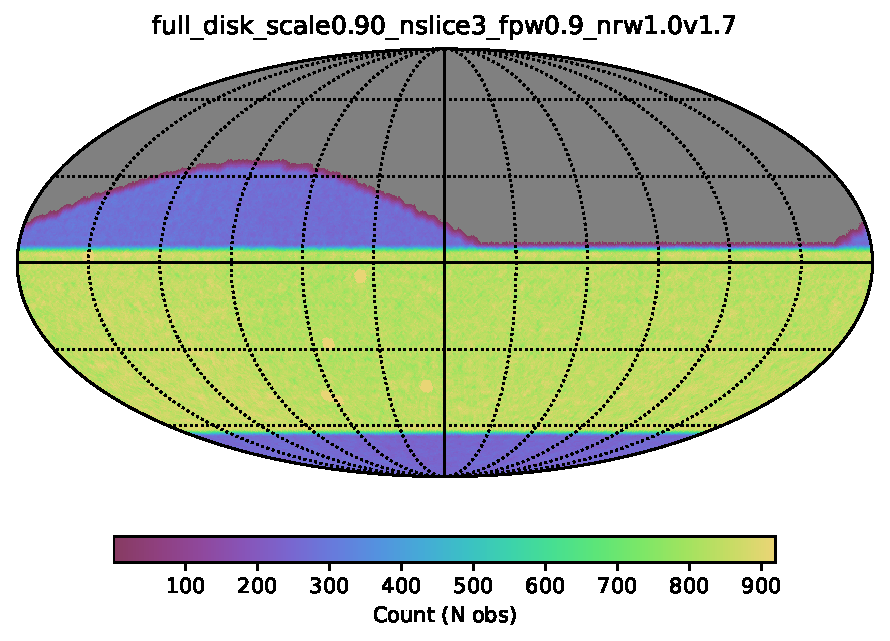
\includegraphics[height=1.25in, width=1.75in]{plots/full_disk_scale0.90_nslice3_fpw0.9_nrw1.0v1.7/full_disk_scale0_90_nslice3_fpw0_9_nrw1_0v1_7_Count_HEAL_SkyMap.pdf}
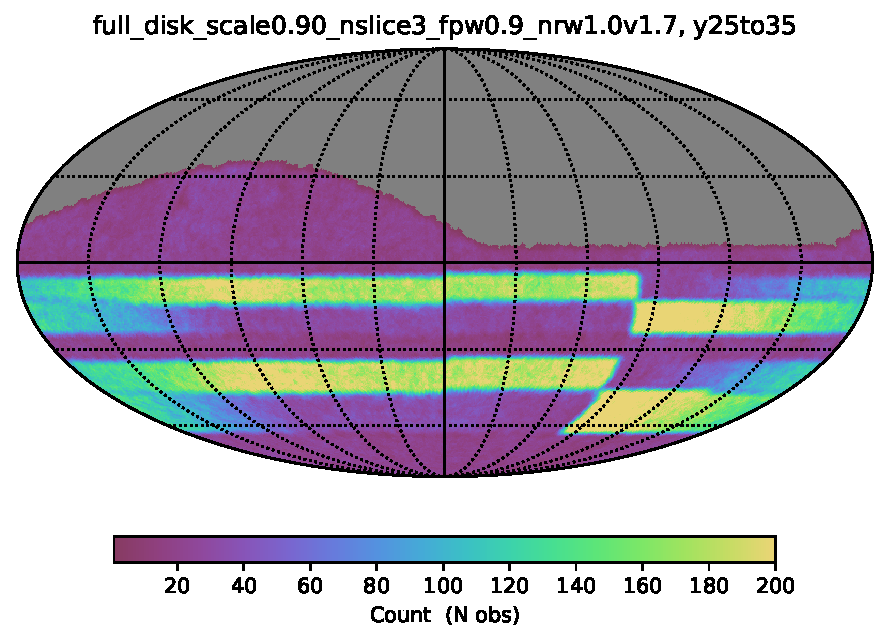
\includegraphics[height=1.25in, width=1.75in]{plots/full_disk_scale0.90_nslice3_fpw0.9_nrw1.0v1.7/full_disk_scale0_90_nslice3_fpw0_9_nrw1_0v1_7_Count_night_gt_913_125000_and_night_lt_1278_375000_and_note_not_like_DD_HEAL_SkyMap.pdf}
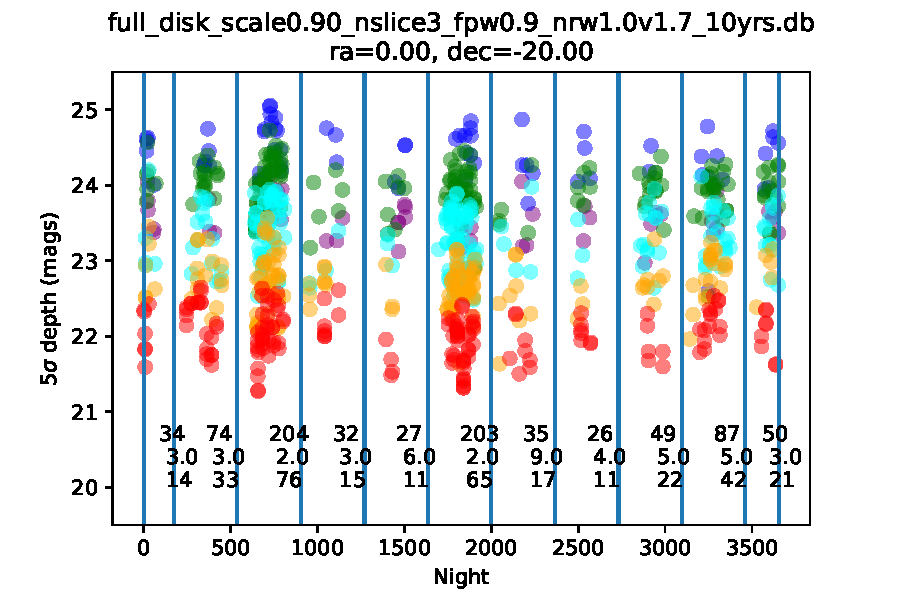
\includegraphics[height=1.25in, width=1.75in]{plots/full_disk_scale090_nslice3_fpw09_nrw10v17_spotc.pdf}
\caption{Like Figure~\ref{fig:classics} but for a footprint that treats the Galactic plane as part of the WFD region. }
\end{figure}


\begin{figure}
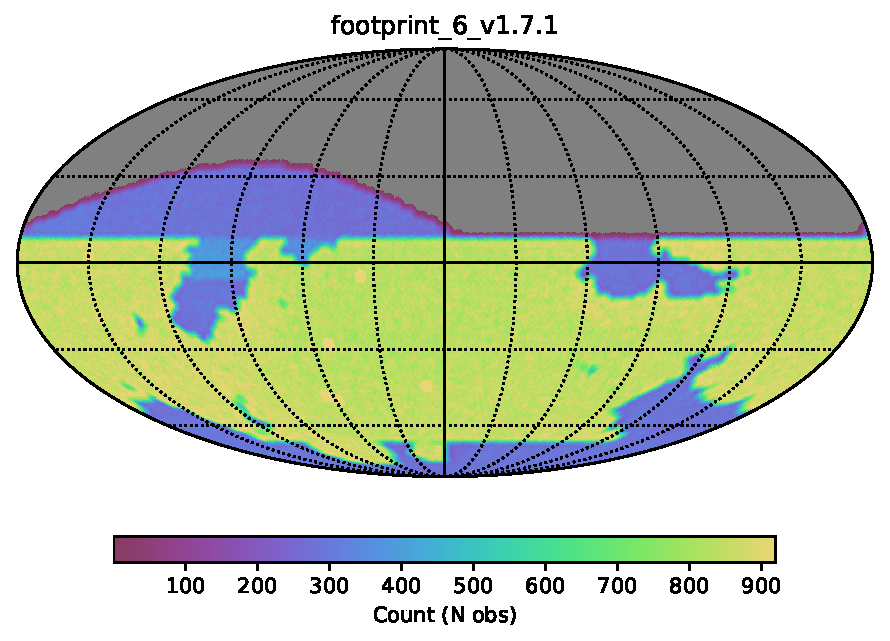
\includegraphics[height=1.25in, width=1.75in]{plots/footprint_6_v1.7.1/footprint_6_v1_7_1_Count_HEAL_SkyMap.pdf}
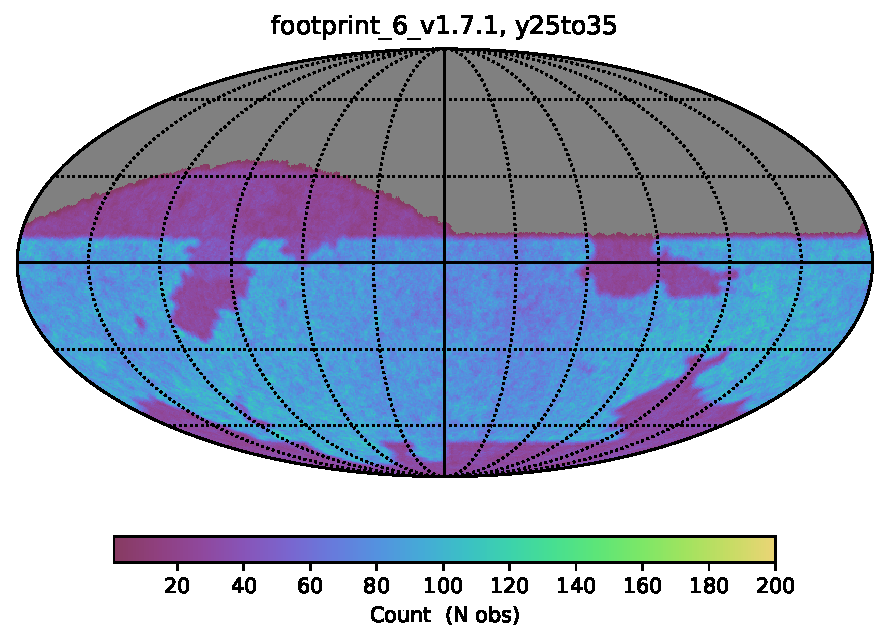
\includegraphics[height=1.25in, width=1.75in]{plots/footprint_6_v1.7.1/footprint_6_v1_7_1_Count_night_gt_913_125000_and_night_lt_1278_375000_and_note_not_like_DD_HEAL_SkyMap.pdf}
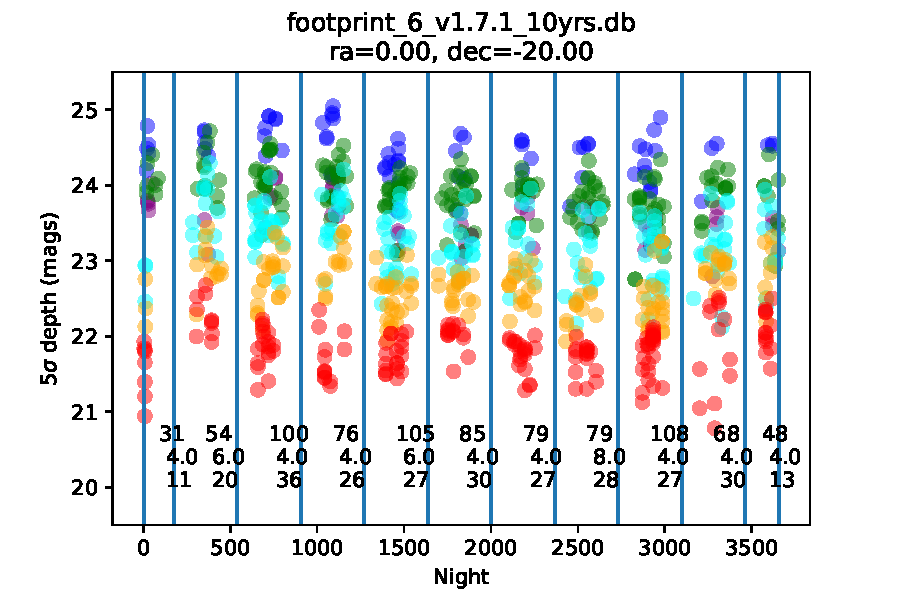
\includegraphics[height=1.25in, width=1.75in]{plots/footprint_6_v171_spotc.pdf} \\

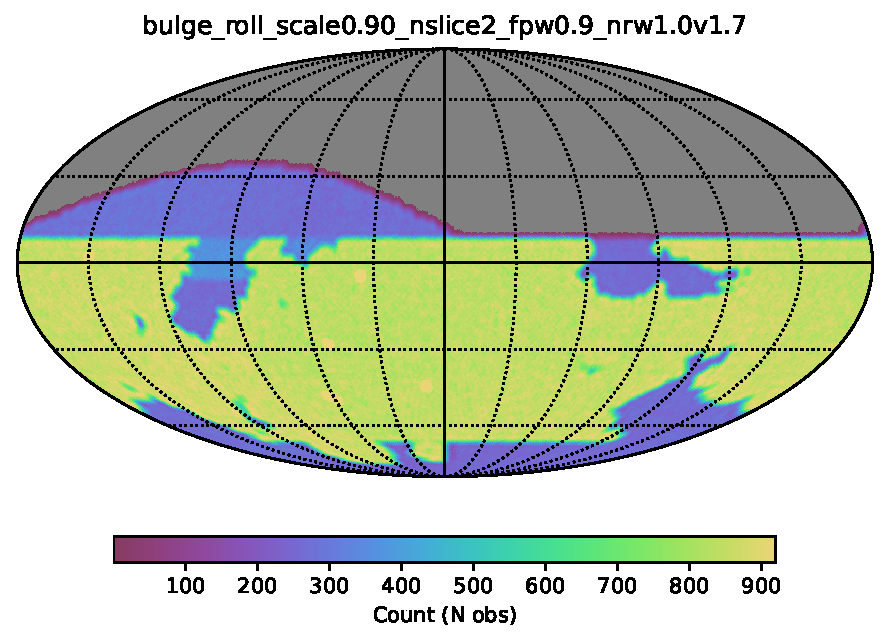
\includegraphics[height=1.25in, width=1.75in]{plots/bulge_roll_scale0.90_nslice2_fpw0.9_nrw1.0v1.7/bulge_roll_scale0_90_nslice2_fpw0_9_nrw1_0v1_7_Count_HEAL_SkyMap.pdf}
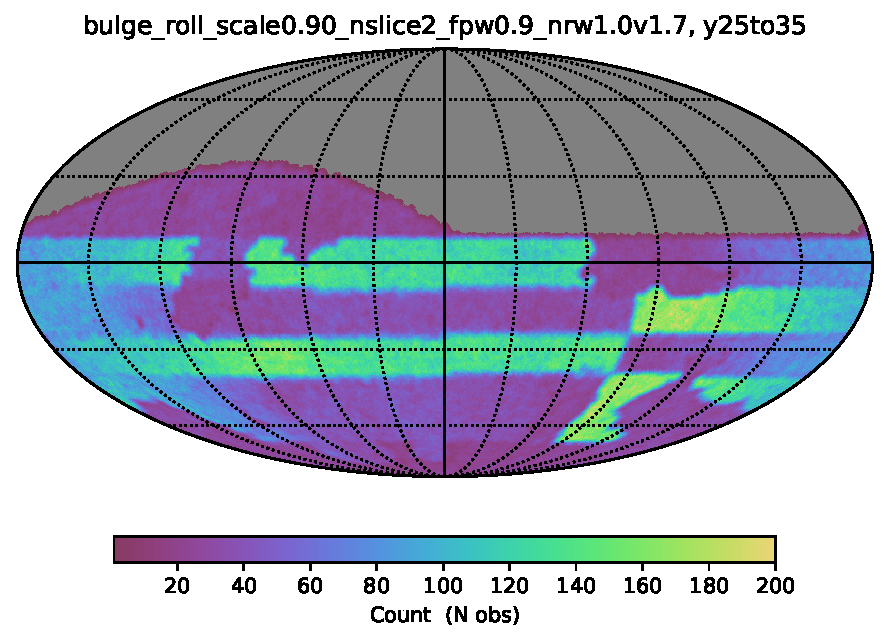
\includegraphics[height=1.25in, width=1.75in]{plots/bulge_roll_scale0.90_nslice2_fpw0.9_nrw1.0v1.7/bulge_roll_scale0_90_nslice2_fpw0_9_nrw1_0v1_7_Count_night_gt_913_125000_and_night_lt_1278_375000_and_note_not_like_DD_HEAL_SkyMap.pdf}
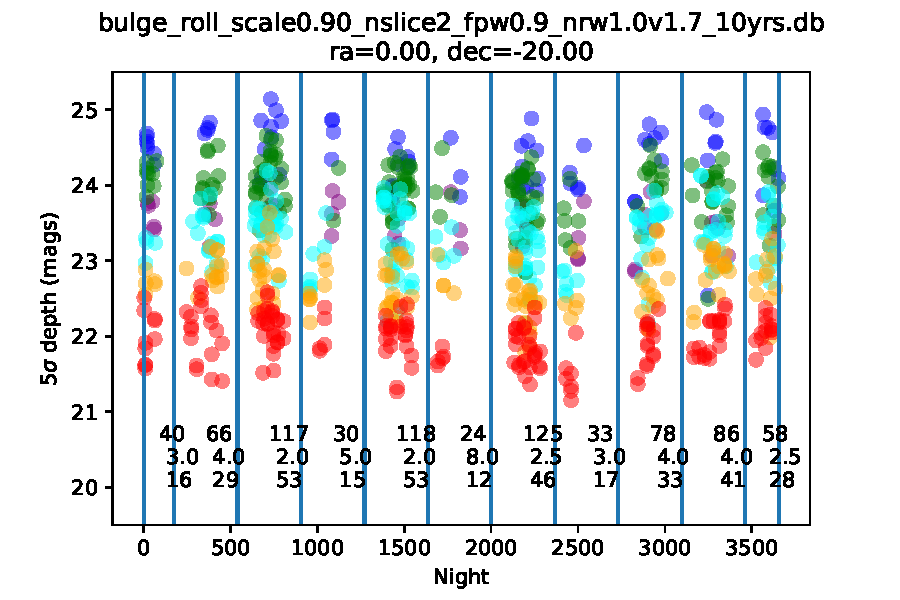
\includegraphics[height=1.25in, width=1.75in]{plots/bulge_roll_scale090_nslice2_fpw09_nrw10v17_spotc.pdf} \\
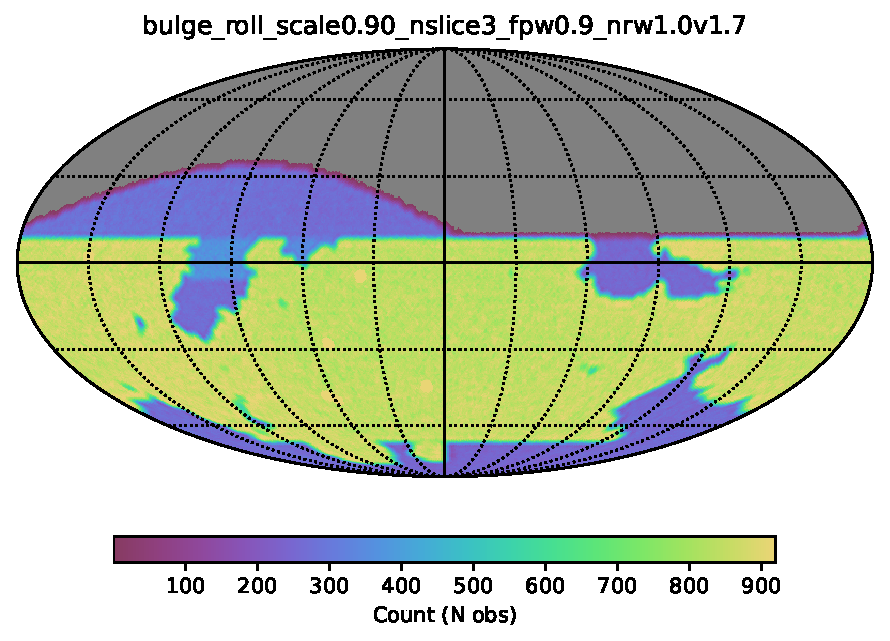
\includegraphics[height=1.25in, width=1.75in]{plots/bulge_roll_scale0.90_nslice3_fpw0.9_nrw1.0v1.7/bulge_roll_scale0_90_nslice3_fpw0_9_nrw1_0v1_7_Count_HEAL_SkyMap.pdf}
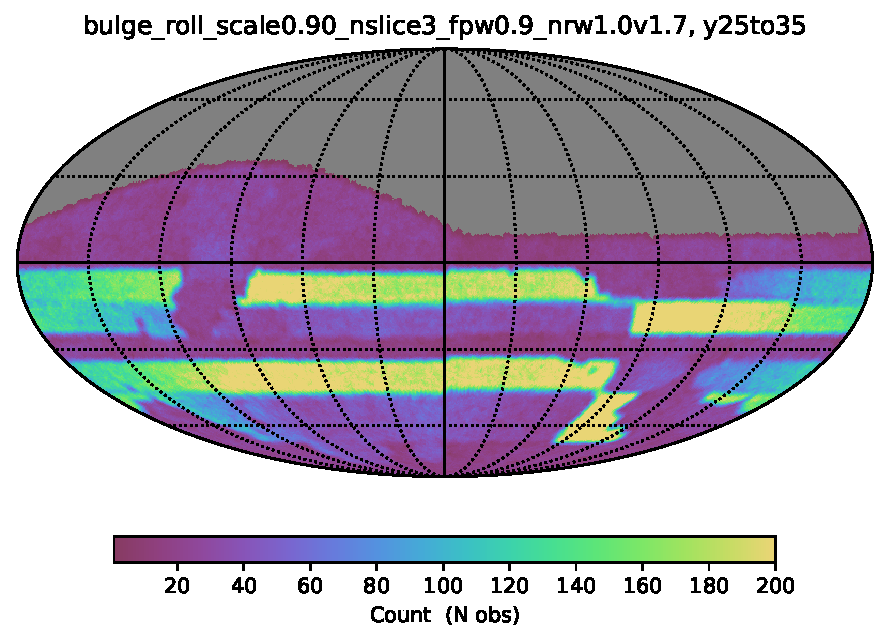
\includegraphics[height=1.25in, width=1.75in]{plots/bulge_roll_scale0.90_nslice3_fpw0.9_nrw1.0v1.7/bulge_roll_scale0_90_nslice3_fpw0_9_nrw1_0v1_7_Count_night_gt_913_125000_and_night_lt_1278_375000_and_note_not_like_DD_HEAL_SkyMap.pdf}
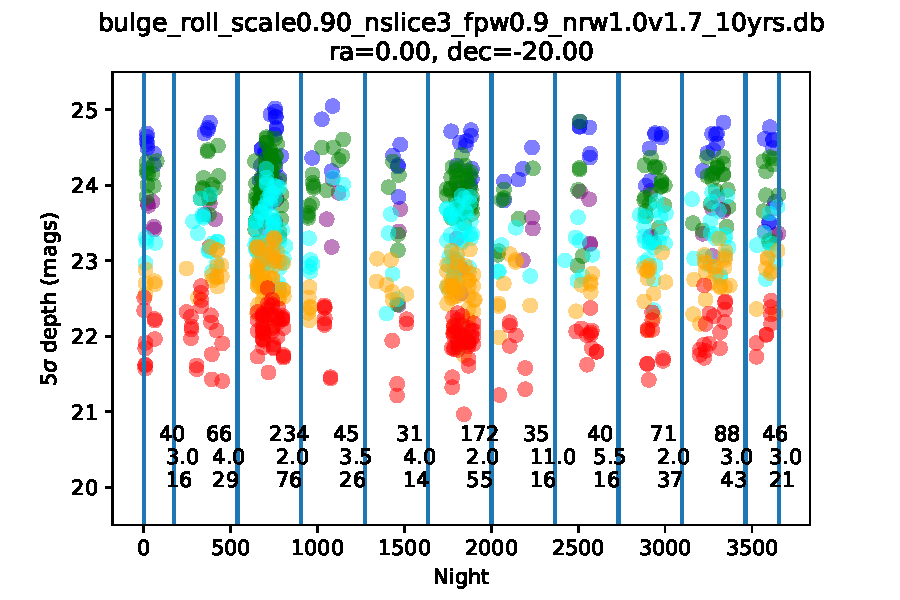
\includegraphics[height=1.25in, width=1.75in]{plots/bulge_roll_scale090_nslice3_fpw09_nrw10v17_spotc.pdf} \\
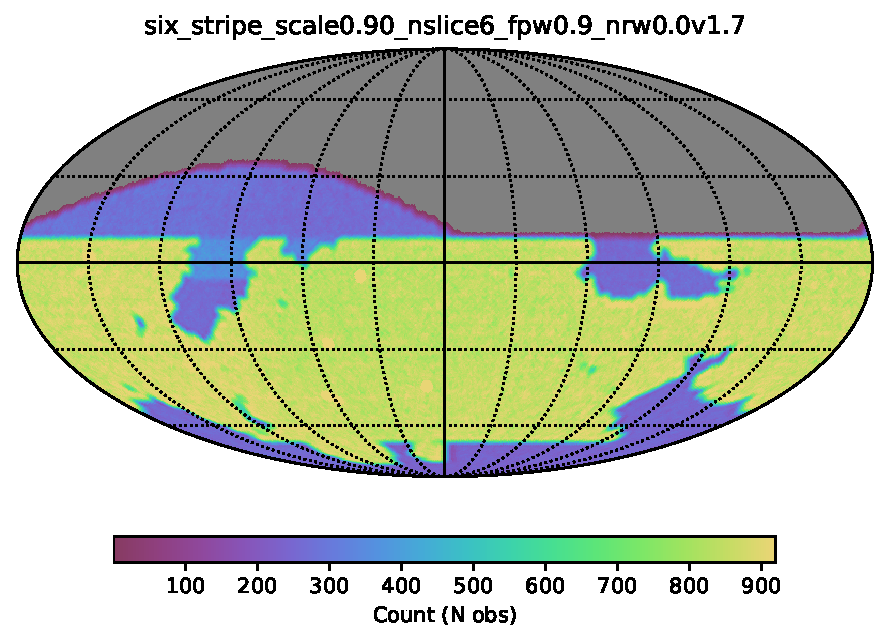
\includegraphics[height=1.25in, width=1.75in]{plots/six_stripe_scale0.90_nslice6_fpw0.9_nrw0.0v1.7/six_stripe_scale0_90_nslice6_fpw0_9_nrw0_0v1_7_Count_HEAL_SkyMap.pdf}
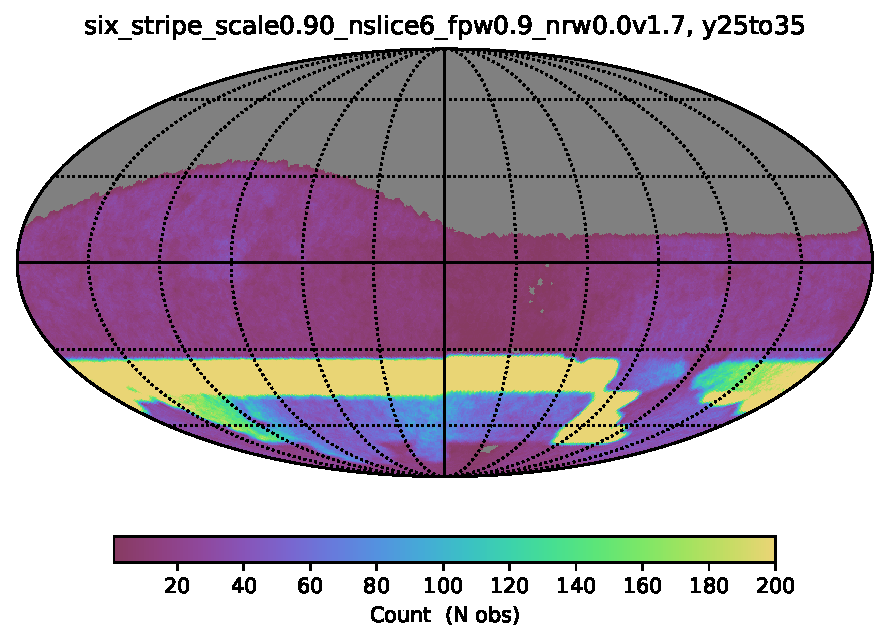
\includegraphics[height=1.25in, width=1.75in]{plots/six_stripe_scale0.90_nslice6_fpw0.9_nrw0.0v1.7/six_stripe_scale0_90_nslice6_fpw0_9_nrw0_0v1_7_Count_night_gt_913_125000_and_night_lt_1278_375000_and_note_not_like_DD_HEAL_SkyMap.pdf}
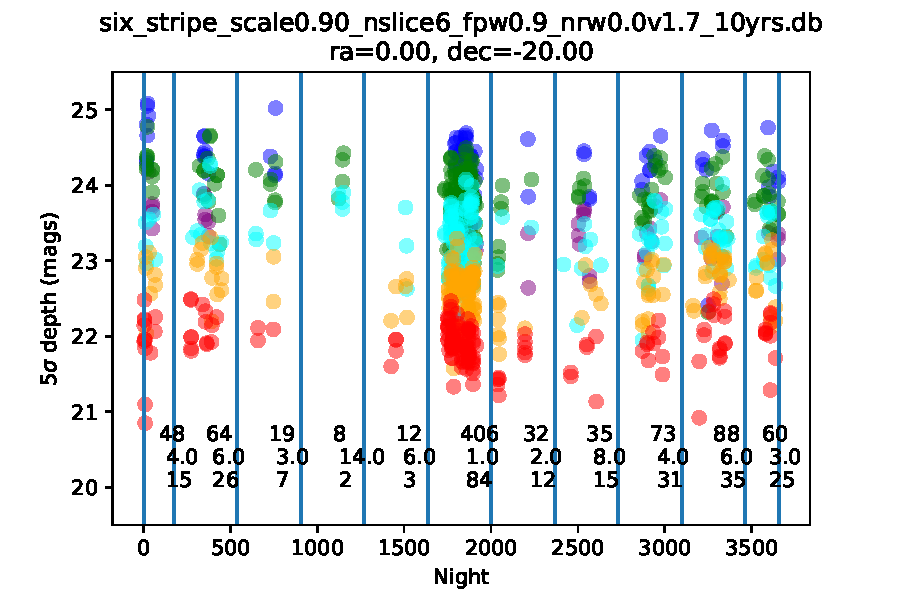
\includegraphics[height=1.25in, width=1.75in]{plots/six_stripe_scale090_nslice6_fpw09_nrw00v17_spotc.pdf} 
\caption{Like Figure~\ref{fig:classics}, but for a compromise footprint that includes the bulge, a plane bridge, and the Magellanic Clouds as part of WFD. Here we have also included an extreme rolling with 6 bands. This results in a point on the sky having one high cadence season and 5 low cadence seasons. Note that such extreme rolling means that there will be multiple years where northern telescopes have little to no chance to follow up Rubin alerts.}
\end{figure}


A note of caution about the number of SNe metric--I'm not convinced it includes Galactic dust, so there may be some additional sensitivity to survey footprint that isn't taken into account yet.


\begin{table}
\begin{tabular}{lccccc}

 Run Name &  N SNe &  Fast Microlensing &  Slow Microlensing &  max N &  min N \\
\toprule

baseline\_nexp2 &             30894.34 &                    0.15 &                    0.95 &     95 &     75 \\
rolling\_nslice2 &             39372.89 &                    0.15 &                    0.95 &    151 &     28 \\
rolling\_nslice3 &             39516.23 &                    0.16 &                    0.95 &    220 &     31 \\


\hline
full\_disk &             27770.56 &                    0.44 &                    0.95 &     97 &     67 \\
full\_disk\_nslice2 &             38607.76 &                    0.42 &                    0.95 &    153 &     35 \\
full\_disk\_nslice3 &             39104.88 &                    0.39 &                    0.95 &    204 &     26 \\
                                
                                   
\hline
footprint\_6 &             22330.58 &                    0.44 &                    0.95 &    108 &     54 \\
bulge\_roll\_nslice2 &             37674.05 &                    0.42 &                    0.95 &    125 &     24 \\
bulge\_roll\_nslice3 &             38094.83 &                    0.40 &                    0.95 &    234 &     31 \\
six\_stripe\_nslice6 &             41416.11 &                    0.34 &                    0.95 &    406 &      8 \\
\hline
\end{tabular}
\end{table}





\begin{figure}
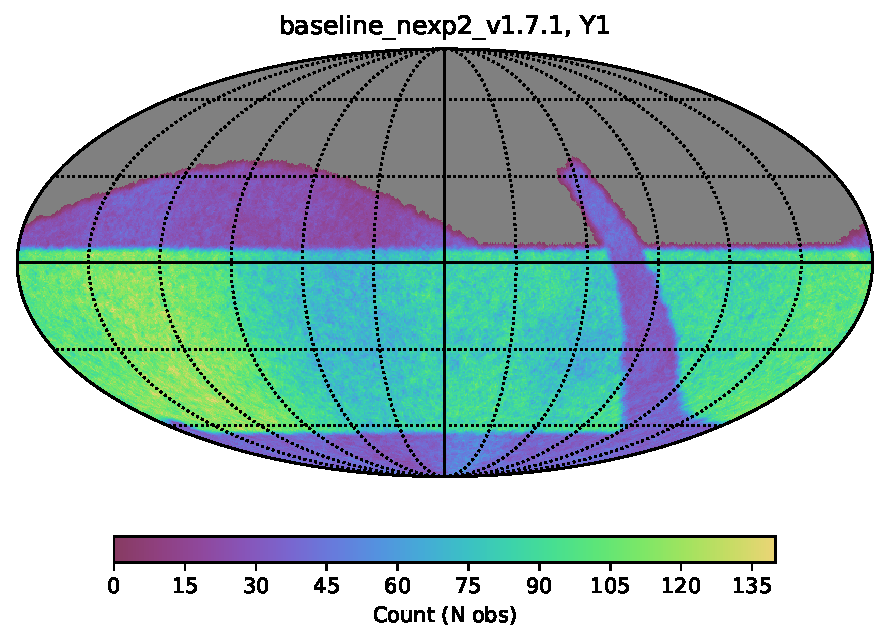
\includegraphics[width=1.75in]{plots/yearly_release/baseline_nexp2_v1_7_1_Count_night_lt_365_and_note_not_like_DD_HEAL_SkyMap.pdf}
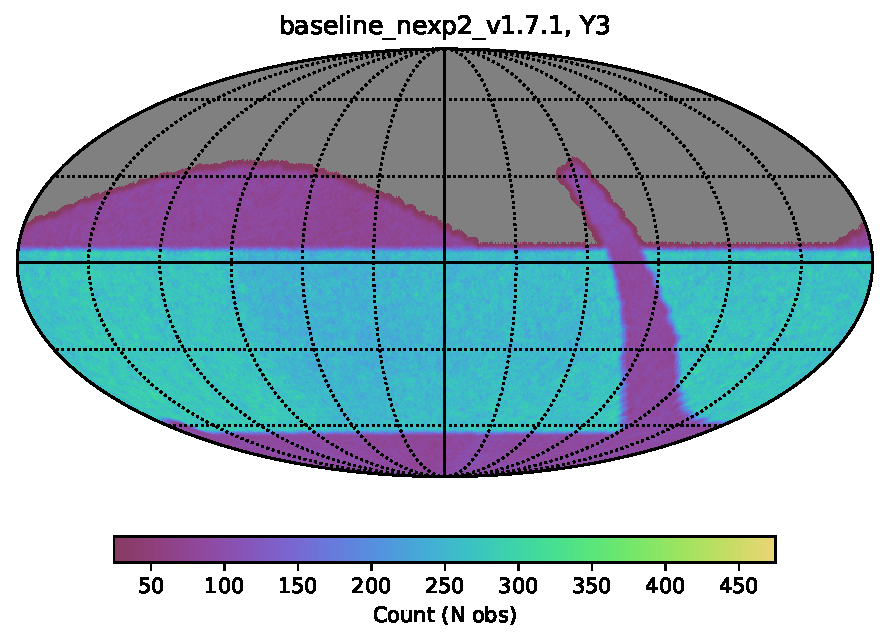
\includegraphics[width=1.75in]{plots/yearly_release/baseline_nexp2_v1_7_1_Count_nightlt1095_and_note_not_like_DD_HEAL_SkyMap.pdf}
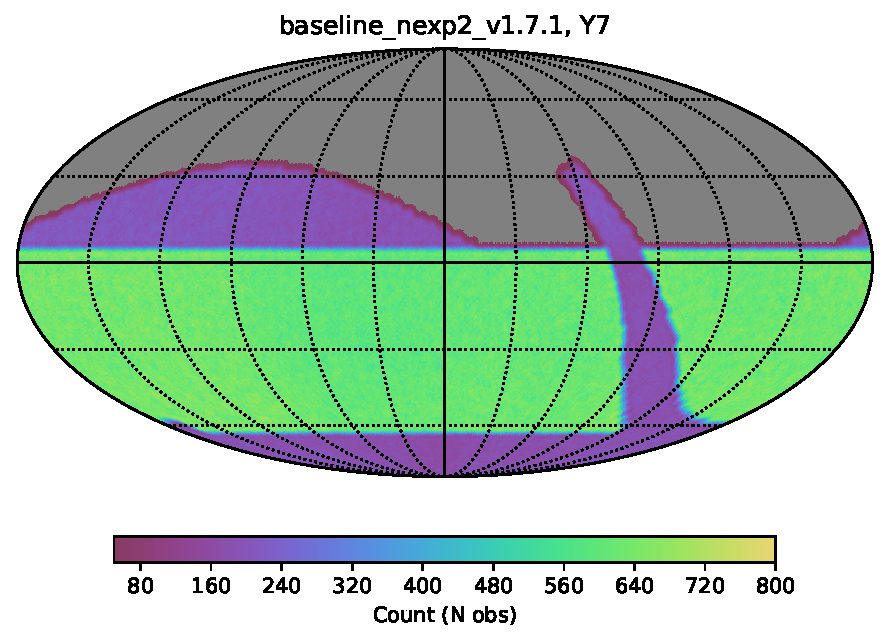
\includegraphics[width=1.75in]{plots/yearly_release/baseline_nexp2_v1_7_1_Count_night_lt_2556_and_note_not_like_DD_HEAL_SkyMap.pdf}\\
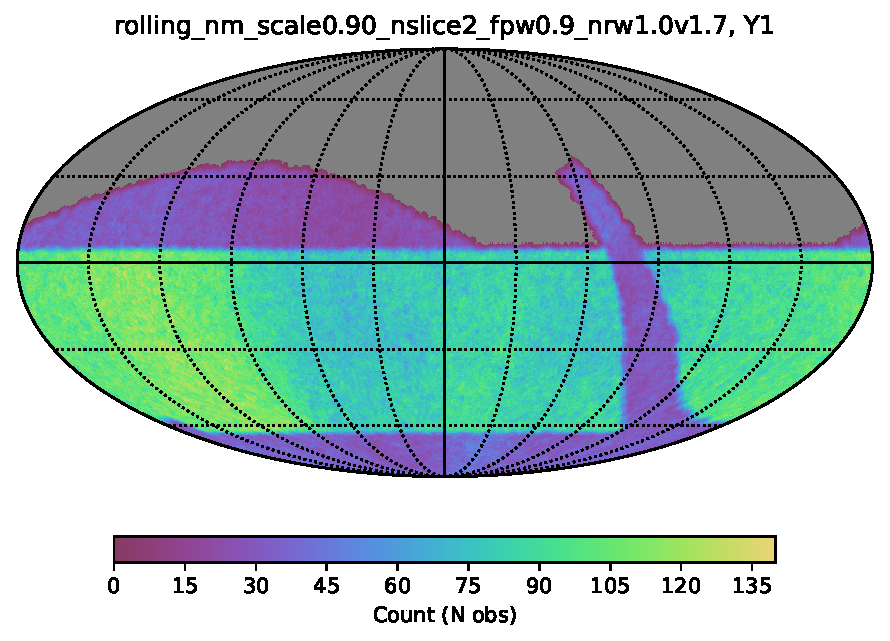
\includegraphics[width=1.75in]{plots/yearly_release/rolling_nm_scale0_90_nslice2_fpw0_9_nrw1_0v1_7_Count_night_lt_365_and_note_not_like_DD_HEAL_SkyMap.pdf}
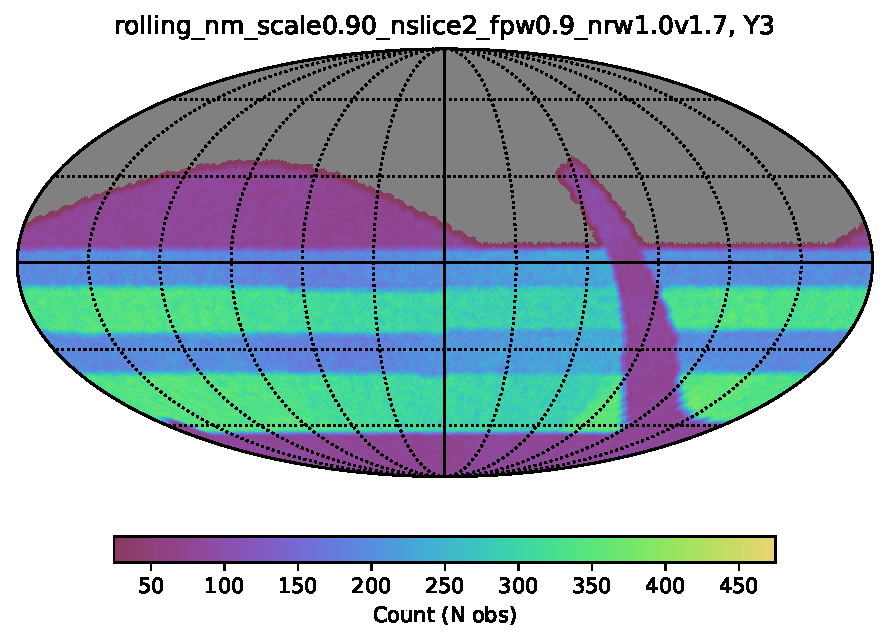
\includegraphics[width=1.75in]{plots/yearly_release/rolling_nm_scale0_90_nslice2_fpw0_9_nrw1_0v1_7_Count_nightlt1095_and_note_not_like_DD_HEAL_SkyMap.pdf}
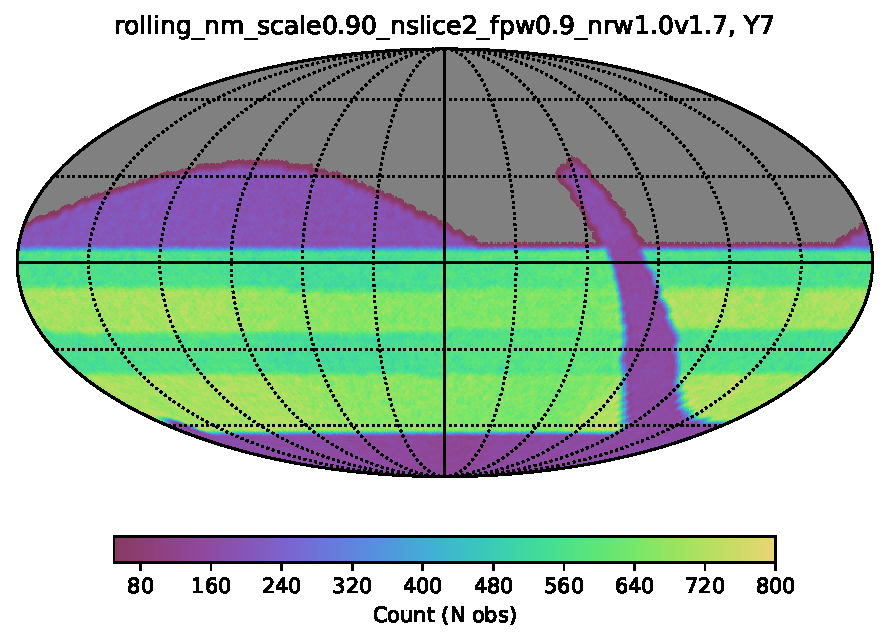
\includegraphics[width=1.75in]{plots/yearly_release/rolling_nm_scale0_90_nslice2_fpw0_9_nrw1_0v1_7_Count_night_lt_2556_and_note_not_like_DD_HEAL_SkyMap.pdf}\\
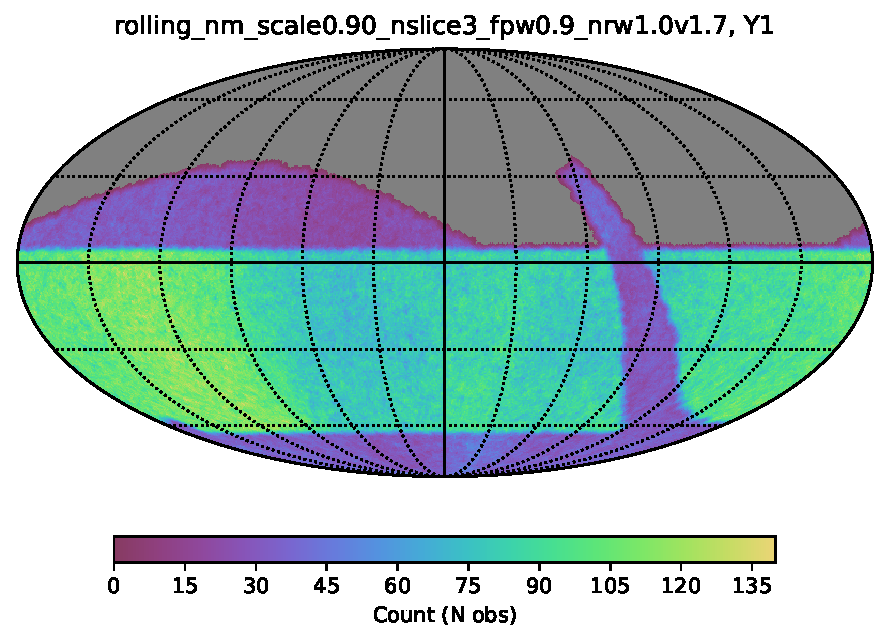
\includegraphics[width=1.75in]{plots/yearly_release/rolling_nm_scale0_90_nslice3_fpw0_9_nrw1_0v1_7_Count_night_lt_365_and_note_not_like_DD_HEAL_SkyMap.pdf}
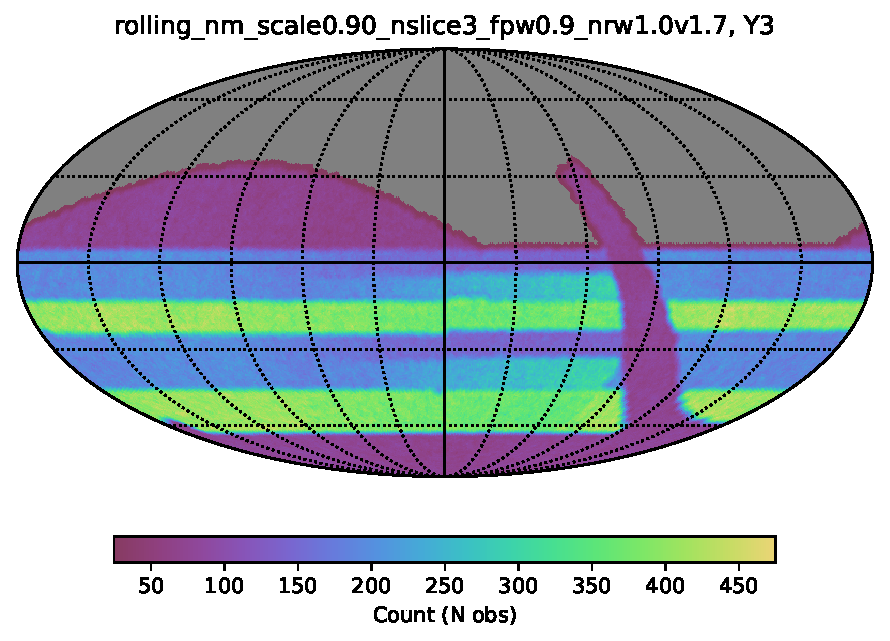
\includegraphics[width=1.75in]{plots/yearly_release/rolling_nm_scale0_90_nslice3_fpw0_9_nrw1_0v1_7_Count_nightlt1095_and_note_not_like_DD_HEAL_SkyMap.pdf}
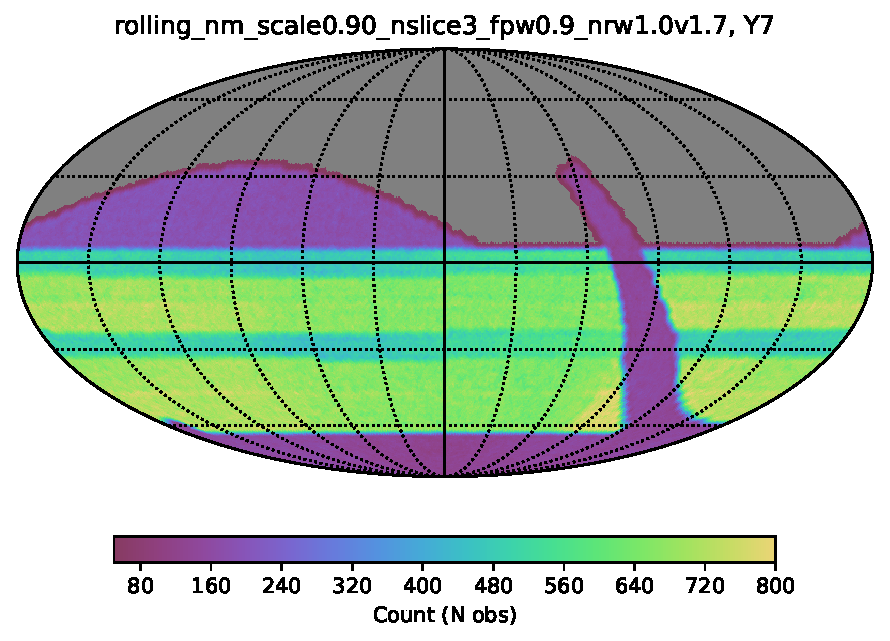
\includegraphics[width=1.75in]{plots/yearly_release/rolling_nm_scale0_90_nslice3_fpw0_9_nrw1_0v1_7_Count_night_lt_2556_and_note_not_like_DD_HEAL_SkyMap.pdf}

\end{figure}

One consequence rolling cadence--data releases will not be uniform! XXX--add plots showing state of survey at various years

\section{Conclusions}

When does rolling work well? 

When is the rolling impact minimal?

If a transient is somewhat recovered in the baseline, going to rolling cadence may not add much boost since some seasons go to lower cadence.

If transient recovery requires higher cadence blue filter coverage. All of the above simulations favor observing in redder filters in bright time. xxx-insert figure showing hourglass. 


Note, rolling itself does not modify the season length.  We can modify the season length, but these simulations all use the same 6-month season. There have been proposals to have ``accordion cadence" for the DDFs. While this is easy to do for DDFs, having an extended season in the broad areas could be difficult to implement. One would need to take care to extend the season length without introducing undesirable side-effects such as forcing blue filters in bright time.


The number of Type Ia SNe takes a big hit moving from the baseline footprint to the compromise footprint\_6, but even modest rolling on footprint\_6 generates more SNe than the baseline. 

The fraction of slow microlensing events does not seem to be sensitive to footprint or rolling. The events are so long that they almost always get discovered.

Slow microlensing events are very sensitive to both footprint and rolling strategy. Note we do not expect the recovery fraction to exceed $\sim50\%$\ simply because many events will happen when the bulge is not observable. 



% Include all the relevant bib files.
% https://lsst-texmf.lsst.io/lsstdoc.html#bibliographies
\bibliographystyle{yahapj}
\bibliography{local,lsst,lsst-dm,refs_ads,refs,books}

% Make sure lsst-texmf/bin/generateAcronyms.py is in your path
\section{Acronyms} \label{sec:acronyms}
\input{acronyms.tex}

\end{document}
